%!TEX root = notes.tex
% Template for PLoS
% Version 1.0 January 2009
%
% To compile to pdf, run:
% latex plos.template
% bibtex plos.template
% latex plos.template
% latex plos.template
% dvipdf plos.template

\documentclass[10pt]{article}

% amsmath package, useful for mathematical formulas
\usepackage{amsmath}
% amssymb package, useful for mathematical symbols
\usepackage{amssymb}

% graphicx package, useful for including eps and pdf graphics
% include graphics with the command \includegraphics
\usepackage{graphicx}

% cite package, to clean up citations in the main text. Do not remove.
\usepackage{cite}

\usepackage{color}

% Use doublespacing - comment out for single spacing
%\usepackage{setspace}
%\doublespacing

% Text layout
\topmargin 0.0cm
\oddsidemargin 0.5cm
\evensidemargin 0.5cm
\textwidth 16cm
\textheight 21cm

% Bold the 'Figure #' in the caption and separate it with a period
% Captions will be left justified
\usepackage[labelfont=bf,labelsep=period,justification=raggedright]{caption}

% Use the PLoS provided bibtex style
\bibliographystyle{plos2009}

% Remove brackets from numbering in List of References
\makeatletter
\renewcommand{\@biblabel}[1]{\quad#1.}
\makeatother


% Leave date blank
\date{}

\pagestyle{myheadings}
%% ** EDIT HERE **
% bussproofs for deduction style proofs
\usepackage{bussproofs}
% xy-pic for diagrams
\usepackage[all]{xy}
% subcaption
\usepackage{subcaption}
% hyperref
\usepackage{hyperref}
\hypersetup{colorlinks=true,
linkcolor=[rgb]{.67 .27 .27},
citecolor=[rgb]{.09 .29 .54},
urlcolor=[rgb]{.09 .29 .54}}
% color table cells http://goo.gl/ZmpJv
\usepackage[table]{xcolor}
%rotate text in table http://goo.gl/Lb4Zd
\usepackage{rotating}
% todo notes see http://www.texample.net/tikz/examples/todo-notes/
\usepackage[colorinlistoftodos]{todonotes}
% for comments
\usepackage{verbatim}
% personal package
\usepackage{crs}
%semantics
\usepackage{latexsym}
\usepackage{stmaryrd}

% set depth for table of contents
% http://tex.stackexchange.com/a/17879/6784
% http://tex.stackexchange.com/a/11669/6784
\setcounter{tocdepth}{4}
\setcounter{secnumdepth}{0}

%% ** EDIT HERE **
%% PLEASE INCLUDE ALL MACROS BELOW

% Set autoref text
% http://tex.stackexchange.com/a/36576/6784
\renewcommand*{\figureautorefname}{Fig.}
\renewcommand*{\equationautorefname}{Eq.}
\renewcommand*{\tableautorefname}{Table}

%% END MACROS SECTION


\begin{document}

% Add Figure, Table prefixes to references
% http://tex.stackexchange.com/a/6063/6784
\let\ref\autoref

% Table of contents
% http://tex.stackexchange.com/a/7357/6784
%\pagebreak
\pagenumbering{gobble}
\tableofcontents
\listoffigures
%\listoftables
\pagebreak
\pagenumbering{arabic}

% Title must be 150 characters or less
%!TEX root = ../notes.tex
\begin{flushleft}
{\Large
\textbf{Notes on type-free vs simply typed lambda calculi and their categorical semantics}
}
% Insert Author names, affiliations and corresponding author email.
\\
Cameron Smith$^{1, \ast}$,
Ximo Pechuan$^{1}$
% Daniel Biro$^{1}$,
% Aviv Bergman$^{1,2,3,4, \ast}$
\\
\bf{1} Department of Systems and Computational Biology, Albert Einstein College of Medicine, Bronx, NY, USA
% \bf{2} Dominick P. Purpura Department of Neuroscience,
% \bf{3} Department of Pathology, Albert Einstein College of Medicine, Bronx, NY, USA
% \bf{4} Santa Fe Institute, 1399 Hyde Park Road, Santa Fe, NM 87501, USA
\\
$\ast$ E-mail: cameron.smith@med.einstein.yu.edu
\end{flushleft}


\listoftodos

% Please keep the abstract between 250 and 300 words
%\section{Abstract}
%\input{tex/abstract.tex}

% Please keep the Author Summary between 150 and 200 words
% Use first person. PLoS ONE authors please skip this step.
% Author Summary not valid for PLoS ONE submissions.
%\section{Author Summary}

%%erase/comment out this section once some real comments are present
%\begin{comment}
\section{Example usage of todo notes}
This is a sentence about which a comment is made in the margin\todo[fancyline, size=\small, color=green!40]{This is an example usage of a todonote todo note.}\todo[color=blue!40]{Todonote with a different color and having the standard thin line back to the same point in the text as the previous note.}. This is an example of a placeholder for a figure:
\missingfigure{insert figure of ...}
\todo[inline, color=red!50]{You can also have inline todonotes.}
This is a paragraph about which a comment is made with no line pointing back into the text\todo[noline]{A note with no line back to the text.}.
%\end{comment}


%\section{Introduction}
%\input{tex/introduction.tex}

% Results and Discussion can be combined.

%\section{Functional closure}
\section{Simply typed lambda calculus}
The simply typed lambda calculus ($\lambda$-calculus) is essentially equivalent to a cartesian closed category in a sense we can make precise. Both are languages in which it is possible to express transformations via functions between objects with operations that express pairing, projection, and application.

The simply typed lambda calculus is made up of types, terms and equations as follows:
\begin{enumerate}
\item{Types:}
\begin{align*}
&\mbox{basic types: } A, B, \ldots\\
&\mbox{product types: } A \times B, \ldots\\
&\mbox{function types: } A \rightarrow B, \ldots
\end{align*}
\item{Terms:}
\begin{align*}
&\mbox{variables: } x, y, z, \ldots \colon A \mbox{ for each type } A,\\
&\mbox{constants: } a \colon A, b \colon B, \mbox{ for each type},\\
&\mbox{products: }\langle a, b \rangle \colon A \times B \mbox{ for } a:A \mbox{ and } b:B,\\
&\mbox{first projection: }\mbox{fst}(c) \colon A \mbox{ for } c \colon A \times B,\\
&\mbox{second projection: }\mbox{snd}(c) \colon A \mbox{ for } c \colon A \times B,\\
&\mbox{application: }ca \colon B \mbox{ for } c \colon A \rightarrow B \mbox{ and } a \colon A,\\
&\mbox{abstraction: }\lambda x. b \colon A \rightarrow B \mbox{ for } x \colon A \mbox{ and } b \colon B
\end{align*}
\item{Equations:}
\begin{align*}
            \mbox{fst}(\langle a, b \rangle) &= a\\
            \mbox{snd}(\langle a, b \rangle) &= b\\
            \langle \mbox{fst}(c), \mbox{snd}(c) \rangle &= c\\
            (\lambda x.b)a &= b[a/x]\\
            \lambda x.cx &= c, \mbox{ $x$ not in $c$ }\\
            \lambda x.b &= \lambda y.b [y/x], \mbox{ no $y$ in $b$ }
\end{align*}
\end{enumerate}
A variable reference $x$ is said to be \emph{bound} if it is inside of an abstraction binding $x$. For example $\lambda x. x$ is a term in which $x$ is bound whereas $\lambda y. x y$ is a term in which $x$ is unbound or \emph{free} and $y$ is bound. A term is said to be \emph{closed} if there are no unbound variables. Therefore, $\lambda x.x$ is a closed term whereas $\lambda y.xy$ is not. Terms are identified according to the equivalence relation $a \sim b$ generated by the equations above.

\section{Categorical semantics for the simply typed lambda calculus}
A category can be associated to any particular instantiation of the lambda calculus with given types, variables and constants. To any such language $\mathcal{L}$ satisfying the defining equations of the simply typed lambda calculus, a cartesian closed category of types $\mathcal{C}(\mathcal{L})$ is determined by the following identifications
\begin{enumerate}
\item{objects: } types
\item{morphisms: } terms $c \colon A \rightarrow B$ that are identified for $c \sim c'$ given by the equivalence relation determined by the defining equations of $\lambda$-calculus. Two equivalence classes of terms $[a], [b]$ may be identified $[a] = [b]$ if and only if the terms they represent are equivalent, which is to say that  $\mathcal{L} \vdash a = b$.
\item{identities: } $1_A = \lambda x.x$ where $x \colon A$
\item{morphism composition: } $c \circ b = \lambda x.c(bx)$
\end{enumerate}
The unit laws, associativity of composition, the existence of products, terminal objects, and exponential objects can be verified from this set of identifications to prove that the category $\mathcal{C}(\mathcal{L})$ is cartesian closed.

If we refer to the set of basic types, terms, and equations as a \emph{theory}, $\mathcal{L}$, in the $\lambda$-calculus, then $\mathcal{C}(\mathcal{L})$ is the cartesian closed category presented by the generators (types and terms) and relations (equations) stated by the $\lambda$-calculus over $\mathcal{L}$. A model of a such a theory $\mathcal{L}$ in the $\lambda$-calculus in a cartesian closed category $\mathcal{C}$ is given by an assignment of types and terms in $\mathcal{L}$ to objects and morhphisms in $\mathcal{C}$:
\begin{align*}
X \mbox{ basic type } &\leadsto \llbracket X \rrbracket\\
b \colon A \rightarrow B \mbox{ basic term } &\leadsto \llbracket b \rrbracket \colon \llbracket A \rrbracket \rightarrow \llbracket B \rrbracket
\end{align*}
which can be naturally extended to the other types and terms that are built upon these. Moreover the equations associated to the theory $\mathcal{L}$ are required to be satisfied so that:
\begin{align*}
\mathcal{L} \vdash [a]=[b] \colon A \rightarrow B \Longrightarrow \llbracket a \rrbracket = \llbracket b \rrbracket \colon \llbracket A \rrbracket \rightarrow \llbracket B \rrbracket
\end{align*}
This semantic association between a theory $\mathcal{L}$ in $\lambda$-calculus and models of such theories in cartesian closed categories is referred to as \emph{denotational semantics} for the $\lambda$-calculus. Indeed, there is a logical completeness theorem associated to such semantics stating that for any theory $\mathcal{L}$ in the $\lambda$-calculus equivalence of terms is mirrored precisely by equivalence of the semantic interpretations of those terms in all models for $\mathcal{L}$ in cartesian closed categories. Although we will not expose the proof of this theorem here, it is important to note that it is not sufficient to consider only the category $\mathbf{Sets}$ as then there are some equations that hold among the models in that restricted context that cannot be proved in a theory of $\lambda$-calculus.

%!TEX root = ../notes.tex
\section{The type-free lambda calculus and its categorical semantics}
The type-free lambda calculus can be seen as a special case of the simply-typed lambda calculus in which the set of basic types is restricted to contain only a single type. With the typing constraint imposed by having multiple types removed, it should be possible to perform self-application as in the term $\lambda x. xx$. If the second occurence of $x$ in this term has type $D$ and the whole term $xx$ has type $D$ then the first occurrence of $x$ in the term $xx$ must be construable as having type $[D \rightarrow D]$. A presentation of the type-free theory, $\mathbb{T}$, can then be given in a manner analogous to that of the simply typed lambda calculus~\cite{Awodey2000}:
\begin{enumerate}
\item{Types:}
\begin{align*}
&\mbox{one basic type: } D\\
\end{align*}
\item{Terms:}
\begin{align*}
&\mbox{variables: } x,y,z, \ldots \colon D\\
&\mbox{constants: } i \colon [D \rightarrow D] \rightarrow D,\,\, r \colon D \rightarrow [D \rightarrow D]\\
\end{align*}
\item{Equations:}
\begin{align*}
            \lambda x. ri(x) &= \lambda x.x\\
            \lambda x. ir(x) &= \lambda x.x
\end{align*}
\end{enumerate}
On this basis, we are led to the requirement that
$$
[D \rightarrow D] \cong D,
$$
which is a particular instantiation of a more general phenomenon referred to as a recursive domain equation. The process by which $[D \rightarrow D]$ is formed in the first place is via the internal Hom bifunctor $F \equiv [-,-] \colon \mathcal{C}^{op} \times \mathcal{C} \rightarrow \mathcal{C}$ on a category $\mathcal{C}$, which thereby restricts consideration for the purpose of finding denotational semantics for the type-free $\lambda$-calculus to categories $\mathcal{C}$ that are closed since this is a necessary condition for it to posses the necessary structure to define the internal Hom bifunctor. In this light, the solution $D$ to the equation $[D,D] \cong D$ is a fixed point $F(D,D) \cong D$ of the internal Hom bifunctor on some category $\mathcal{C}$.

Given these restrictions, it is obvious that it will not be sufficient in the search for non-trivial models of the type-free theory of the $\lambda$-calculus to restrict consideration to the category $\mathbf{Sets}$ because in such a category $F$ has a fixed point $D$ only when $D$ is the one element set: $D = \{*\}$. However, $\mathbb{T}$ does not necessarily prove $\lambda y.ir(y)=\lambda y.y$, which would be true for $D = \{*\}$. Because something provable in $\mathbf{Sets}$ is not necessarily provable in the type-free $\lambda$-calculus there is no sense in which semantics in the category $\mathbf{Sets}$ could be complete with respect to the type-free $\lambda$-calculus.

We will very briefly sketch the solution to this particular problem and refer to other sources for caveats and details~\cite{Barendregt1985,Smyth1982,Freyd1990,Abramsky1995,Cattani2007}. In order to remedy this situation Scott eventually introduced \emph{domains}, which can be viewed as \emph{continuous lattices} (this construction appears with minor modifications with respect to the purpose of the present exposition in terms of various other closely related kinds of objects and their associated categories such as complete partial orders and complete lattices among others). A continuous lattice is a complete \todo{Include appropriate definitions from lattice theory (e.g. lattice, meet, join, completeness, etc.)} lattice $D$ such that
$$
\forall d \in D, d = \bigvee \left\{ \bigwedge U | d \in U, U \mbox{ Scott-open}, U \subseteq D \right\}
$$
where \emph{Scott-open} refers to a subset $U$ of a domain $D$ that is upward closed in the sense that if $\bigvee \Delta \in U$ for a directed subset $\Delta \subseteq D$ then $U \cap \Delta \neq \emptyset$ and Scott-continuous functions are required to be monotonic and preserve least upper bounds of directed subsets of their domains. These continuous lattices can be equivalently characterized in topological terms as $T_0$-spaces in which every continuous function $f \colon P \rightarrow D$ from a subspace $P \subseteq S$ can be extended to a Scott-continuous function $\hat{f} \colon S \rightarrow D$.

Domains of this form taken as objects and Scott-continuous functions between them taken as morphisms form cartesian closed categories where the internal-hom (i.e. exponential) objects were naturally themselves not sets but complete lattices of Scott-continuous functions. Since these form a cartesian closed category they could be used as described above to provide semantics for the simply-typed $\lambda$-calculus. However, categories of domains can also be constructed that have reflexive objects, $D_\infty$, which solve the recursive domain equation $F(D_{\infty},D_{\infty})=D_{\infty}$ that arises naturally as described above in the analysis of the type-free $\lambda$-calculus since, there, objects serve both as arguments and as functions that can be applied to such arguments.

The way in which such solutions $D_\infty$ are constructed is via a generalization of the least fixed-point of a continuous function. A continous function $f \colon D \rightarrow D$ may have fixed-points $x$ such that $f(x)=x$. The least fixed-point for such a continuous function $f$ is then given by
$$
fix(f) = \bigvee_{n \in \omega} f^n(\bot)
$$
Now, we would like to extend this notion to the internal-hom bifunctor $F \equiv [-,-] \colon \mathcal{C}^{op} \times \mathcal{C} \rightarrow \mathcal{C}$ for $\mathcal{C}$ a category of continuous lattices and Scott-continuous functions. Given domains $D$ and $E$ as objects in such a category, we can define an \emph{embedding-projection pair} from $D$ to $E$ as a pair of Scott-continuous functions $i \colon D \rightarrow E$ and $r \colon E \rightarrow D$ such that $r \circ i = id_D$ and $i \circ r \leq id_E$ where the relation of order on functions is given pointwise. Reflexive domains are given by inverse limits (or projective limits, which are specializations of limits, as opposed to colimits, in category theory) of sequences of projections $r_n$ given by:
\begin{align*}
&D_0 = \mbox{ some object, $D$, in } \mathcal{C},\\
&D_1 = [D_0 \rightarrow D_0],\\
&D_{n+1} = [D_n \rightarrow D_n],\\
&(r_n \colon D_{n+1} \rightarrow D_n)_{n \in \omega}.
\end{align*}
The fact that a suitable choice for the initial embedding-projection pair $\langle i_0, r_0 \rangle$ ultimately requires that the limit of the above sequence of projections coincide with the colimit of the sequence of embeddings
$$
(i_n \colon D_{n} \rightarrow D_{n+1})_{n \in \omega}.
$$
It is eventually possible to obtain
$$
\lim_{\leftarrow} (D_n, r_n) \cong D_\infty \cong \lim_{\rightarrow} (D_n, i_n).
$$
and this particular construction of $D_{\infty}$ provides a fixed-point $\text{FIX}(F)$ so that $F(D_{\infty},D_{\infty}) = D_{\infty}$ solves the given recursive domain equation associated to the untyped $\lambda$-calculus. This allows us to interpret the terms of the untyped lambda calculus as being the objects and morphisms $D_{\infty}$ and $[D_{\infty},D_{\infty}]$ respectively, which are now seen to be one and the same since $D_{\infty} \cong D_{\infty}^{D_{\infty}}$.



%\section{Discussion}
%\input{tex/discussion.tex}

% Do NOT remove this, even if you are not including acknowledgments
\section{Acknowledgments}
The authors would like to thank Jay Sulzberger and Noson Yanofsky for helpful discussions.

%\section{References}
% The bibtex filename
\bibliography{bib/books,bib/papers}
\pagebreak
% You may title this section "Methods" or "Models".
% "Models" is not a valid title for PLoS ONE authors. However, PLoS ONE
% authors may use "Analysis"

\section{Background}
\subsection{Categories}\todo{Some of this section is ``textbook'' material taken from planetmath.org. It is a helpful reference to definitions for reviewers.}
%!TEX root = ../notes.tex
An intuitive picture to which one can anchor intuition when thinking in category theoretic terms is presented in \ref{fig:intextdiag}. In category theory, one can always consider the duality between the intrinsic structure of \emph{objects} and the manner in which that intrinsic structure can be expressed externally in terms of patterns of constraints placed upon the relationships between \emph{morphisms} among objects.

\begin{figure}
\begin{center}
\noindent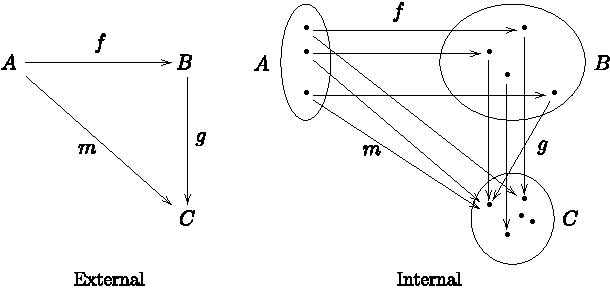
\includegraphics[width=0.8\columnwidth]{fig/intextdiag.pdf}
\end{center}
\caption{In the external diagram on the left one simply considers \emph{objects} such as $A$,$B$, and $C$ and morphisms between them $f$, $g$, and $m$. The internal perspective, which in this case is specific to the category of $\mathbf{Sets}$, demonstrates the particular manner in which the equation $g \circ f = m$ may be satisfied in terms of the internal structure of the objects $A$, $B$, and $C$. Of course, in this case there are many other ways of satisfying the given equation; however, there are also questions that can be answered about the relationship between $A$, $B$, and $C$ given either $g \circ f = m$ or $g \circ f \neq m$ without necessarily knowing the particular manner in which either equation is satisfied by the relationships among the internal structures of the objects involved.}
\label{fig:intextdiag}
\end{figure}

A \emph{category} $\mathcal{C}$ consists of the following data:
\begin{enumerate}
\item a class $\operatorname{ob}(\mathcal{C})$ of objects (of $\mathcal{C}$)
\item for each ordered pair $(A,B)$ of objects of $\mathcal{C}$, a collection (we will assume it is
 a set) $\hom(A,B)$ of morphisms from the domain $A$ to the codomain $B$
\item a function $\circ:\hom(A,B)\times\hom(B,C)\to\hom(A,C)$ called composition.
\end{enumerate}

We normally denote $\circ(f,g)$ by $g \circ f$ for morphisms $f,g$. The above data must satisfy the following axioms: for objects $A,B,C,D$,

\textbf{A1}: $\hom(A,B) \cap \hom(C,D)=\emptyset$ whenever $(A,B)\neq (C,D)$, i.e. the intersection is non-trivial only when $A=C$ and $B=D$.

\textbf{A2}: (Associativity) if $f \in \hom(A,B)$, $g\in\hom(B,C)$ and $h\in\hom(C,D)$, $h\circ (g\circ f)=(h\circ g)\circ f$

\textbf{A3}: (Existence of an identity morphism) for each object $A$ there exists an identity morphism $ {}id_{A}\in\hom(A,A)$ such that for every $f\in\hom(A,B)$, $f\circ id_{A}=f$ and $ {}id_{A}\circ g=g$ for every $g \in \hom(B,A)$.

Some examples of categories:
\begin{itemize}
\item \textbf{0} is the empty category with no objects or morphisms, \textbf{1} is the category with one object and one (identity) morphism.
\item If we assume we have a universe $U$ which contains all sets encountered in ``everyday'' mathematics,
\textbf{Set} is the category of all such small sets with morphisms being set functions
\item \textbf{Top} is the category of all small topological spaces with morphisms continuous functions
\item \textbf{Grp} is the category of all small groups whose morphisms are group homomorphisms
\end{itemize}

\textbf{Remark}.  If $\hom(A,B)$ in the second condition above is not required to be a set (but a class), we usually call $\mathcal{C}$ a \emph{large category}.

\subsubsection{Initial and terminal objects}
An {\em initial object} in a category $\mathcal{C}$ is an object $A$ in $\mathcal{C}$ such that, for every object $X$ in $\mathcal{C}$, there is exactly one morphism $A \longrightarrow X$. A {\em terminal object} in a category $\mathcal{C}$ is an object $B$ in $\mathcal{C}$ such that, for every object $X$ in $\mathcal{C}$, there is exactly one morphism $X \longrightarrow B$. A {\em zero object} in a category $\mathcal{C}$ is an object $0$ that is both an initial object and a terminal object. All initial objects (respectively, terminal objects, and zero objects), if they exist, are isomorphic in $\mathcal{C}$.

\subsubsection{Functors}
Given two categories $\mathcal{C}$ and $\mathcal{D}$, a covariant\ {\em functor} $T:\mathcal{C}\to\mathcal{D}$ consists of an assignment for each object $X$ of $\mathcal{C}$ an object $T(X)$ of $\mathcal{D}$ (i.e. a ``function'' $T:{\rm Ob}(\mathcal{C})\to{\rm Ob}(\mathcal{D})$) together with an assignment for every morphism $f\in{\rm Hom}_{\mathcal{C}}(A,B)$, to a morphism $T(f)\in{\rm Hom}_{\mathcal{D}}(T(A),T(B))$, such that:
\begin{itemize}
\item $T(1_A) = 1_{T(A)}$ where $1_X$ denotes the identity morphism on the object $X$ (in the respective category).
\item $T(g \circ f) = T(g)\circ T(f)$, whenever the composition $g\circ f$ is defined.
\end{itemize}

A contravariant functor $T :\mathcal{C}\to\mathcal{D}$ is just a covariant functor $T:\mathcal{C}^{\rm op}\to\mathcal{D}$ from the opposite category.  In other words, the assignment reverses the direction of maps.  If $f\in{\rm Hom}_{\mathcal{C}}(A,B)$, then $T(f)\in{\rm Hom}_{\mathcal{D}}(T(B),T(A))$ and $T(g\circ f) = T(f)\circ T(g)$ whenever the composition is defined (the domain of $g$ is the same as the codomain of $f$).

Given a category $\mathcal{C}$ and an object $X$ we always have the functor $T : \mathcal{C}\to{\bf Sets}$ to the category of sets defined on objects by $T(A) = {\rm Hom}(X, A)$.  If $f : A \to B$ is a morphism of $\mathcal{C}$, then we define $T(f) : {\rm Hom}(X,A)\to {\rm Hom}(X,B)$ by $g\mapsto f\circ g$.  This is a covariant functor, denoted by ${\rm Hom}(X,-)$.

Similarly, one can define a contravariant functor ${\rm Hom}(-,X) :\mathcal{C}\to{\bf Sets}$.

\subsubsection{Natural transformations}
Let $\mathcal{C}$ and $\mathcal{D}$ be categories, and let 
$S,T:\mathcal{C}\to\mathcal{D}$ be covariant functors. Then suppose
that for every object $A$ in $\mathcal{C}$ one has a morphism 
$\eta_A :  S(A) \to T(A) $ in $\mathcal{D}$ such that for every morphism 
$\alpha: A \to B$ in $\mathcal{C}$ the following
$$
\xymatrix@+=4pc{S(A) \ar[d]_{S(\alpha)} \ar[r]^{\eta_A} & T(A) \ar[d]^{T(\alpha)} \\
S(B) \ar[r]^{\eta_{B}} & T(B)
}
$$
is commutative.  Then we variously write 
$$
\eta: S \dot{\to} T \quad\mbox{ or }\quad \eta: S\Rightarrow T\quad \mbox{ or } \quad \eta:S\to T
$$
and call $\eta$ a \emph{natural trasformation} from $S$ to $T$.

One may think of a natural transformation $\eta:S\to T$ as a `function' from the class of objects of $\mathcal{C}$ to the class of morphisms of $\mathcal{D}$.

As a first example, for every functor $S:\mathcal{C}\to \mathcal{D}$, we can associate the natural transformation $1_S: S\to S$ (the \emph{identity natural transformation} on $S$) that assigns every object $A$ of $\mathcal{C}$, the corresponding identity morphism $1_{S(A)}$.

Natural transformations are composed in a similar manner to morphisms, but they are nevertheless defined as correspondences between both objects and morphisms as shown in the square commutative diagram depicted above. 

More precisely, given three functors $R,S,T:\mathcal{C}\to \mathcal{D}$, and two natural transformations, $\tau:R\to S$ and $\eta:S\to T$, we define the composition of $\tau$ with $\eta$, written $\eta \bullet \tau$, as a class of morphisms in $\mathcal{D}$ given by 
$$(\eta\bullet \tau)_A := \eta_A\circ \tau_A,$$ for every object $A$ in $\mathcal{C}$.
It is easy to see that $\eta\bullet \tau$ is a natural transformation, since we may ``compose'' two commutative squares and obtain a third one:
$$
\xymatrix@+=4pc{R(A) \ar[d]_{R(\alpha)} \ar[r]^{\tau_A}  & S(A) \ar[d]_{S(\alpha)} \ar[r]^{\eta_A} & T(A) \ar[d]^{T(\alpha)} \ar@{}[dr]|{=} &  
R(A) \ar[d]_{R(\alpha)} \ar[r]^{\eta_A \circ \tau_A} & T(A) \ar[d]^{T(\alpha)} 
\\
R(B) \ar[r]^{\tau_{B}} & S(B) \ar[r]^{\eta_{B}} & T(B) & 
R(B) \ar[r]^{\eta_B \circ \tau_B} & T(B)
}
$$
It is easy to see that the composition ``operation'' on natural transformations is associative:
$$(\zeta\bullet \eta)\bullet \tau = \zeta\bullet (\eta \bullet \tau)$$
for natural transformations $\tau:R\to S$, $\eta:S\to T$, and $\zeta:T\to U$.  In addition, any identity natural transformation acts as a compositional identity: if $\tau:R\to S$ and $\eta:S\to T$, then $$1_S\bullet \tau=\tau \qquad\mbox{ and }\qquad \eta \bullet 1_S = \eta.$$

\subsubsection{Adjoint functors}
Let $\mathcal{C}$ and $\mathcal{D}$ be (small) categories, and let $T:\mathcal{C} \to \mathcal{D}$ and $S:\mathcal{D} \to \mathcal{C}$ be covariant functors. $T$ is said to be a \emph{left adjoint functor} to $S$ (equivalently, $S$ is a \emph{right adjoint functor} to $T$) if there is a natural equivalence
\[
\nu\colon \Hom_{\mathcal{D}}(T(-),-) \overset{\cdot}{\longrightarrow} \Hom_{\mathcal{C}}(-,S(-)).
\]
Here the functor $\Hom_{\mathcal{D}}(T(-),-)$ is a bifunctor $\mathcal{C}\times\mathcal{D}\to\mathbf{Set}$ which is contravariant in the first variable, is covariant in the second variable, and sends an object $(C,D)$ to $\Hom_{\mathcal{D}}(T(C),D)$.  The functor $\Hom_{\mathcal{C}}(-,S(-))$ is defined analogously.

This definition needs additional explanation.  Essentially, it says that for every object $C$ in $\cal{C}$ and every object $D$ in $\cal{D}$ there is a function 
\[
\nu_{C,D} \colon \Hom_{\mathcal{D}}(T(C),D) \overset{\sim}{\longrightarrow} \Hom_{\mathcal{C}}(C,S(D)) 
\]
which is a natural bijection of hom-sets.  Naturality means that if $f\colon C'\to C$ is a morphism in $\mathcal{C}$ and $g\colon D\to D'$ is a morphism in $\mathcal{D}$, then the diagram
\[\xymatrix{
\Hom_{\mathcal{D}}(T(C),D)\ar[dd]_{(Tf,g)}\ar[rr]^{\nu_{C,D}} &&
\Hom_{\mathcal{C}}(C,S(D))\ar[dd]^{(f,Sg)} \\ && \\
\Hom_{\mathcal{D}}(T(C'),D')\ar[rr]^{\nu_{C',D'}} &&
\Hom_{\mathcal{C}}(C',S(D')) \\
}\] 
is a commutative diagram.  If we pick any $h:T(C)\to D$, then we have the equation $$Sg\circ \nu_{C,D}(h)\circ f= \nu_{C',D'}(g\circ h\circ Tf).$$

If $T:\mathcal{C}\to\mathcal{D}$ is a left adjoint of $S:\mathcal{D}\to \mathcal{C}$, then we say that the ordered pair $(T,S)$ is an \emph{adjoint pair}, and the ordered triple $(T,S,\nu)$ an \emph{adjunction} from $\mathcal{C}$ to $\mathcal{D}$, written $$(T,S,\nu):\mathcal{C}\to \mathcal{D},$$ where $\nu$ is the natural equivalence defined above.  

An adjoint to a functor is in some ways like an inverse (as in the case of an adjoint matrix); often formal properties about a functor lead to formal properties of its adjoint (for example the right adjoint to a left-exact functor takes injectives to injectives).  An adjoint to any functor is unique up to natural isomorphism.

\subsubsection{Exponential objects}
Let $A,B$ be objects in a category with finite products $\mathcal{C}$.  An object $E$ in $\mathcal{C}$ is called an \emph{exponential object} from $A$ to $B$ if it satisfies the following conditions:
\begin{itemize}
\item there is a morphism $f:E\times A\to B$, called an \emph{evaluation morphism}
\item for any morphism $g:C\times A\to B$, there is a unique morphism $h:C\to E$ such that $f\circ (h\times 1_A)=g$, where $h\times 1_A:C\times A\to E\times A$ is the product morphism of $h$ and the identity morphism on $A$.
\end{itemize}
The two conditions can be summarized by the following commutative diagram:
\begin{center}
$
\xymatrix@R-=20pt{
E\times A\ar[dr]^f\\
&B\\
C\times A\ar[ur]_g\ar[uu]^{h\times 1_A}
}
$
\end{center}
where $h$ is uniquely determined by $g$.  It is easy to see that any two exponential objects from $A$ to $B$ are isomorphic, hence the existence of an exponential object between two objects is a universal property.  We may write $B^A (\cong E$ above) \emph{the} exponential object from $A$ to $B$.

For example, in the category of sets, $\textbf{Set}$, where products exist between pairs of objects (sets), the exponential from $A$ to $B$ is the set $B^A$, which is defined as the set of all functions from $A$ to $B$.  The evaluation morphism is the function $ev: B^A\times A\to B$ given by $ev(f,a)=f(a)$, where $f\in B^A$ and $a\in A$.  If $g:C\times A\to B$ is any function, then we define $h:C\to B^A$ by $h(c)(a)=g(c,a)$.  Then $ev\circ (h\times 1_A)(c,a)=ev(h(c),a)=h(c)(a)=g(c,a)$, and $ev$ is universal (in the sense of the second condition above).

Since each $h$ is uniquely determined by $g$ in the above definition, and conversely every $h$ determines a $g$ by the formula $g=f\circ (h\times 1_A)$, we have a bijection 
$$
\hom(C\times A,B)\cong \hom(C,B^A).
$$
If an exponential object exists between every pair of objects in category $C$ with finite products, then we say that $C$ \emph{has exponentials}.  According to the bijection above, we see that the functor $\cdot\times A:\mathcal{C}\to \mathcal{C}$ has a right adjoint, namely $\cdot ^A:\mathcal{C}\to\mathcal{C}$, called the \emph{exponential functor}.

%
\subsection{Cartesian closed category}
A category $\mathcal{C}$ with finite products is said to be \emph{Cartesian closed} if each of the following functors has a right adjoint
\begin{enumerate}
\item $\textbf{0}:\mathcal{C}\to \textbf{1}$, where $\textbf{1}$ is the trivial category with one object $0$, and $\textbf{0}(A)=0$
\item the diagonal functor $\delta: \mathcal{C}\to \mathcal{C}\times\mathcal{C}$, where $\delta(A)=(A,A)$, and
\item for any object $B$, the functor $(-\times B):\mathcal{C}\to\mathcal{C}$, where $(-\times B)(A)=A\times B$, the product of $A$ and $B$.
\end{enumerate}
Furthermore, we require that the corresponding right adjoints for these functors to be
\begin{enumerate}
\item any functor $\textbf{1}\to\mathcal{C}$, where $0$ is mapped to an object $T$ in $\mathcal{C}$.  $T$ is necessarily a terminal object of $\mathcal{C}$.  
\item the product (bifunctor) $(-\times -): \mathcal{C} \times \mathcal{C}\to \mathcal{C}$ given by $(-\times -)(A,B)\mapsto A\times B$, the product of $A$ and $B$.
\item for any object $B$, the exponential functor $(-^B):\mathcal{C}\to\mathcal{C}$ given by $(-^B)(A)=A^B$, the exponential object from $B$ to $A$.
\end{enumerate}

In other words, a Cartesian closed category $\mathcal{C}$ is a category with finite products, has a terminal objects, and has exponentials.  It can be shown that a Cartesian closed category is the same as a finitely complete category having exponentials.

Examples of Cartesian closed categories are the category of sets \textbf{Set} ( terminal object: any singleton; product: any Cartesian product of a finite number of sets; exponential object: the set of functions from one set to another)  the category of small categories \textbf{Cat} (terminal object: any trivial category; product object: any finite product of categores; exponential object: any functor category), and every elementary topos.
%
\subsection{Monoidal categories}
A \emph{monoidal category} is a category which has the structure of a monoid, that is, among the objects there is a binary operation which is associative and has an unique neutral or unit element.   Specifically, a category $\mathcal{C}$ is \emph{monoidal} if
\begin{enumerate}
\item there is a bifunctor $\otimes: \mathcal{C}\times\mathcal{C}\to \mathcal{C}$, where the images of object $(A,B)$ and morphism $(f,g)$ are written $A\otimes B$ and $f\otimes g$ respectively,
\item there is an isomorphism $a_{ABC}: (A\otimes B)\otimes C \cong A\otimes (B\otimes C)$, for arbitrary objects $A,B,C$ in $\mathcal{C}$, such that $a_{ABC}$ is natural in $A,B$ and $C$.  In other words,
\begin{itemize}
\item $a_{-BC}: (-\otimes B)\otimes C \Rightarrow -\otimes(B\otimes C)$ is a natural transformation for arbitrary objects $B,C$ in $\mathcal{C}$,
\item $a_{A-C}: (A\otimes -)\otimes C \Rightarrow A\otimes(-\otimes C)$ is a natural transformation for arbitrary objects $A,C$ in $\mathcal{C}$,
\item $a_{AB-}: (A\otimes B)\otimes - \Rightarrow A\otimes(B\otimes -)$ is a natural transformation for arbitrary objects $A,B$ in $\mathcal{C}$,
\end{itemize}
\item there is an object $I$ in $\mathcal{C}$ called the \emph{unit object} (or simply the \emph{unit}),
\item for any object $A$ in $\mathcal{C}$, there are isomorphisms: 
$$l_A: I\otimes A\cong A \qquad \mbox{and} \qquad r_A: A\otimes I\cong A,$$
such that $l_A$ and $r_A$ are natural in $A$: both $l: I\otimes - \Rightarrow -$ and $r: -\otimes I\Rightarrow - $ are natural transformations
\end{enumerate}
satisfying the following commutative diagrams:
\begin{itemize}
\item \emph{unit coherence law}
$$\xymatrix@+=2cm{(A\otimes I)\otimes B \ar[rr]^{a_{AIB}} \ar[dr]_{r_A\otimes 1_B} & & A\otimes (I\otimes B) \ar[dl]^{1_A \otimes r_B} \\ & A\otimes B & }$$
\item \emph{associativity coherence law}
$$\xymatrix@+=2cm{((A\otimes B)\otimes C)\otimes D \ar[rr]^{a_{A\otimes B,C,C}} \ar[d]_{a_{ABC}\otimes 1_D} &&  (A\otimes B)\otimes (C\otimes D) \ar[dd]^{a_{A,B,C\otimes D}} \\ 
(A\otimes (B\otimes C))\otimes D \ar[d]_{a_{A,B\otimes C,D}} && \\
A\otimes ((B\otimes C)\otimes D) \ar[rr]_{1_A\otimes a_{BCD}} && A \otimes (B\otimes (C\otimes D))}$$
\end{itemize}
The bifunctor $\otimes$ is called the \emph{tensor product} on $\mathcal{C}$, and the natural isomorphisms $a,l,r$ are called the \emph{associativity isomorphism}, the \emph{left unit isomorphism}, and the \emph{right unit isomorphism} respectively.

Some examples of monoidal categories are
\begin{itemize}
\item
A prototype is the category of isomorphism classes of vector spaces over a field $\mathbb{K}$, herein the tensor product is the associative operation and the field $\mathbb{K}$ itself is the unit element.
\item
The category of sets is monoidal.  The tensor product here is just the set-theoretic cartesian product, and any singleton can be used as the unit object.
\item
The category of (left) modules over a ring $R$ is monoidal.  The tensor product is the usual tensor product of modules, and $R$ itself is the unit object.
\item
The category of bimodules over a ring $R$ is monoidal.  The tensor product and the unit object are the same as in the previous example.
\end{itemize}
%
\subsection{Symmetric monoidal categories}
A monoidal category $\mathcal{C}$ with tensor product $\otimes$ is said to be \emph{symmetric} if for every pair $A,B$ of objects in $\mathcal{C}$, there is an isomorphism $$s_{AB}:A\otimes B\cong B\otimes A$$ that is natural in both $A$ and $B$ such that the following diagrams are commutative
\begin{enumerate}
\item (\emph{unit coherence for $s$}):
$$\xymatrix@+=2cm{A\otimes I \ar[rr]^{s_{AI}} \ar[dr]_{r_A} & & I\otimes A \ar[dl]^{l_A} \\ & A &}$$
\item (\emph{associativity coherence for $s$}):
$$\xymatrix@+=2cm{ (A\otimes B)\otimes C \ar[rr]^{s_{AB}\otimes 1_C} \ar[d]_{a_{ABC}} & & (B\otimes A)\otimes C \ar[d]^{a_{BAC}} \\ A\otimes (B\otimes C) \ar[d]_{s_{A,B\otimes C}} & & B\otimes (A\otimes C) \ar[d]^{1_B\otimes s_{AC}} \\ (B\otimes C)\otimes A \ar[rr]_{a_{BCA}} & & B\otimes(C\otimes A)
}$$
\item (inverse law):
$$\xymatrix@+=2cm{& B\otimes A \ar[dr]^{s_{BA}} & \\ A\otimes B \ar[ur]^{s_{AB}} \ar@{=}[rr]_{1_{A\otimes B}} && A\otimes B }$$
\end{enumerate}
In the diagrams above, $a,l,r$ are the associativity isomorphism, the left unit isomorphism, and the right unit isomorphism respectively.

Some examples and non-examples of symmetric monoidal categories:
\begin{itemize}
\item The category of sets.  The tensor product is the set theoretic cartesian product, and any singleton can be fixed as the unit object.
\item The category of groups.  Like before, the tensor product is just the cartesian product of groups, and the trivial group is the unit object.
\item More generally, a category with finite products is symmetric monoidal.  The tensor product is the direct product of objects, and any terminal object (empty product) is the unit object.
\item The category of bimodules over a ring $R$ is monoidal.  However, this category is only symmetric monoidal if $R$ is commutative.
\end{itemize}

\textbf{Remark}.  A symmetric monoidal category is a braided monoidal category such that the inverse law: $s_{BA}\circ s_{AB}=1_{A\otimes B}$ holds.

%\section{Figure Legends}

%\section{Tables}

\end{document}

